\section{Auswertung}
\label{sec:Auswertung}

\subsection{Kalibrierung der x-Achse}
Zur Bestimmung des Land\'{e}-Faktors der Elektronen und des Erdmagnetfeldes in Dortmund, werden zunächst die x-Koordinaten in Abbildung \ref{fig:Skizze} zu sehenden Graphen normiert.
\begin{figure}
  \centering
  \begin{subfigure}[b]{0.49\textwidth}
     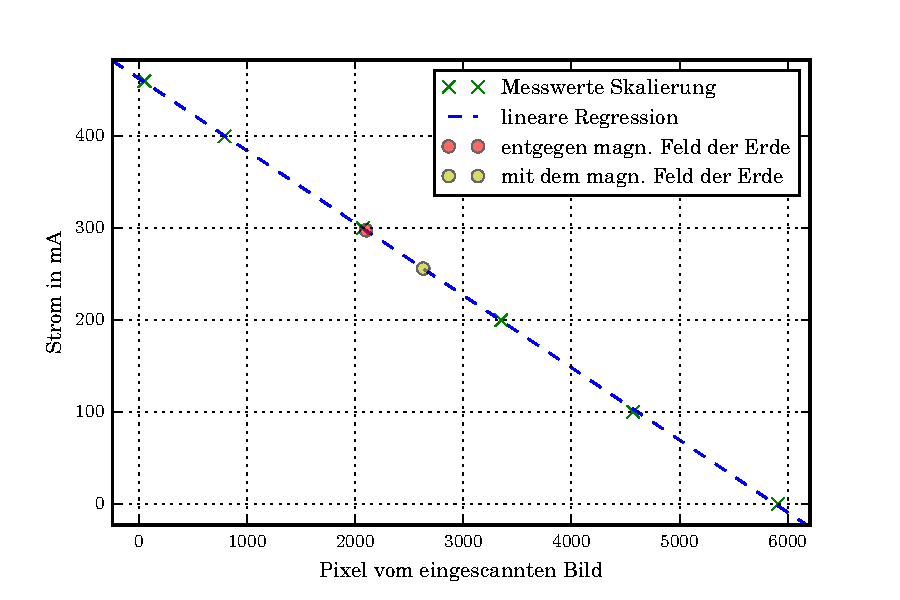
\includegraphics[width=\textwidth]{picture/10MHz.jpg}
     \caption{10.6 MHz}
     \label{fig:10Skiz}
  \end{subfigure}
  \begin{subfigure}[b]{0.49\textwidth}
     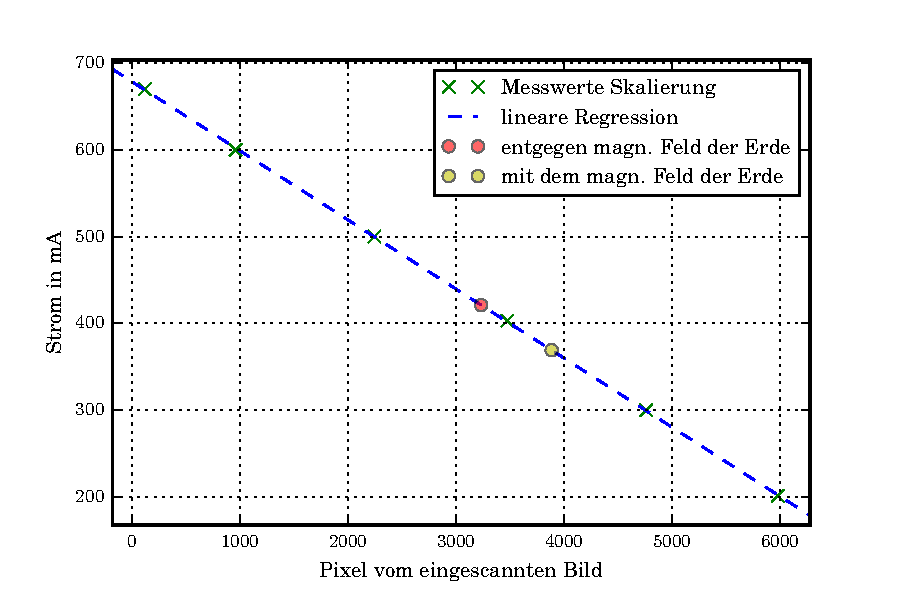
\includegraphics[width=\textwidth]{picture/15MHz.jpg}
     \caption{15.9 MHz}
     \label{fig:15Skiz}
  \end{subfigure}
  \begin{subfigure}[b]{0.49\textwidth}
     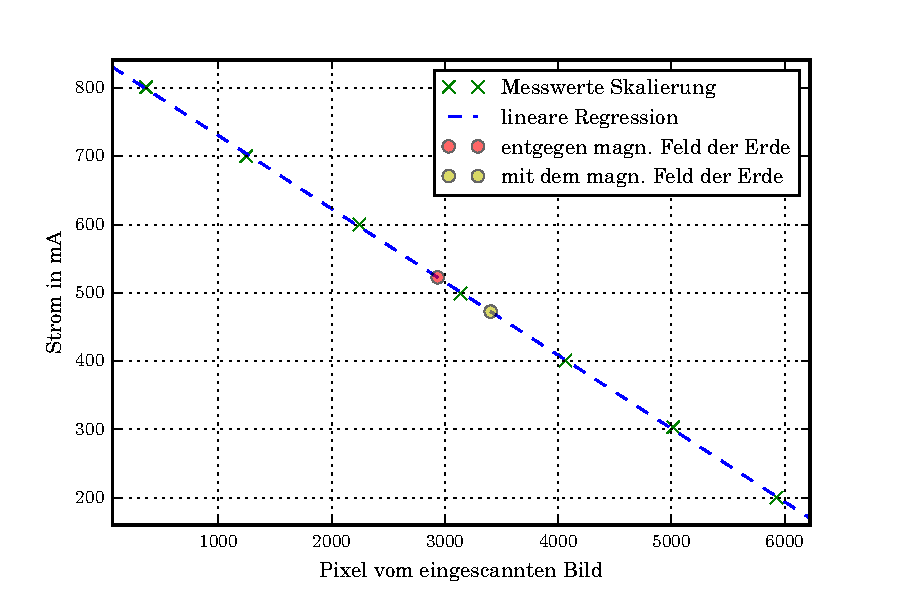
\includegraphics[width=\textwidth]{picture/20MHz.jpg}
     \caption{20.5 MHz}
     \label{fig:20Skiz}
  \end{subfigure}
  \begin{subfigure}[b]{0.49\textwidth}
     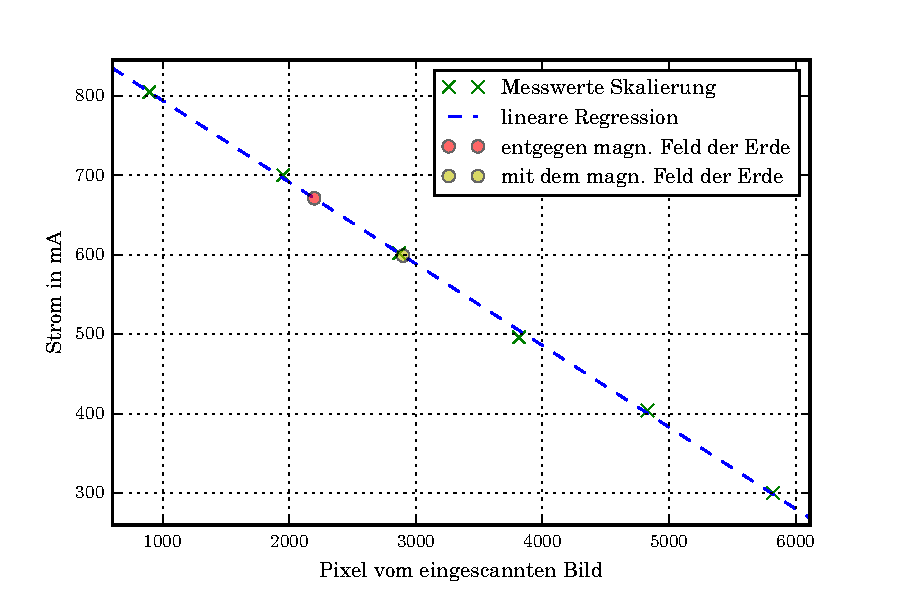
\includegraphics[width=\textwidth]{picture/25MHz.jpg}
     \caption{25.0 MHz}
     \label{fig:25Skiz}
  \end{subfigure}
  \begin{subfigure}[b]{0.49\textwidth}
     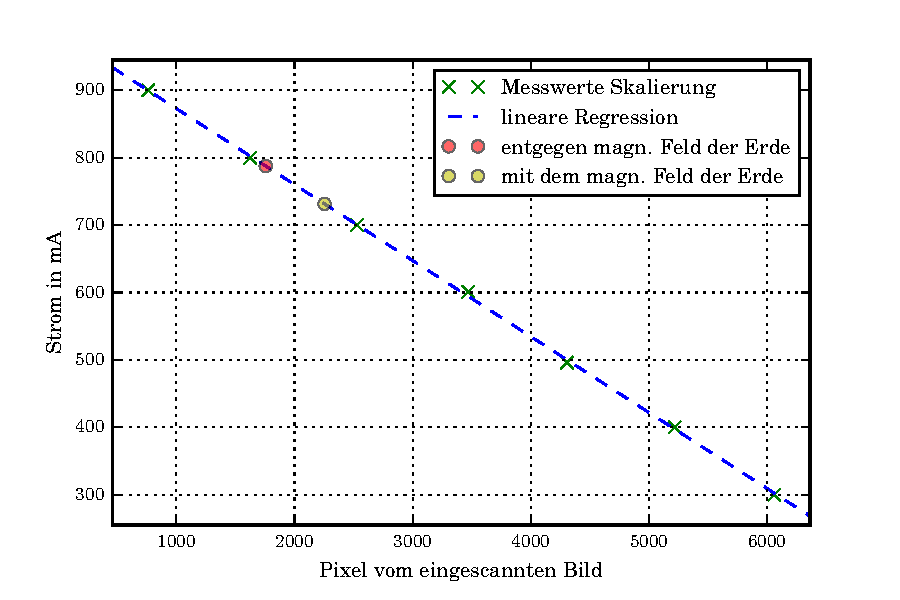
\includegraphics[width=\textwidth]{picture/30MHz.jpg}
     \caption{29.4 MHz}
     \label{fig:30Skiz}
  \end{subfigure}
  \caption{Brückenstrom in abhängigkeit des Spulenstrom für verschiedene $\nu_\text{e}$}
  \label{fig:Skizze}
\end{figure}
Dazu werden die Graphen eingescannt. Mittels eines Bildbearbeitungsprogramm werden die Pixelanzahlen der x-Koordinaten für die gekennzeichneten Spulenströme bestimmt. Die Messwerte sind in Tabelle \ref{tab:Mess1} und \ref{tab:Mess2} aufgetragen. 
\begin{table}
  \centering
  \caption{Pixelzahl in abhängigkeit des Spulenstroms bei $\nu_\text{e}$ = 10-20 MHz}
  \begin{tabular}{c c|c c|c c}
    \toprule
    	$I_{10.6 MHz}$ / mA & Pixel & $I_{15.9 MHz}$ / mA & Pixel & $I_{20.5 MHz}$ / mA & Pixel \\    
    \midrule
	0   & 5911 & 201 & 5980 & 200 & 5928 \\
	100 & 4572 & 300 & 4763 & 303 & 5018 \\
	200 & 3351 & 403 & 3477 & 401 & 4064 \\
	300 & 2070 & 500 & 2245 & 499 & 3138 \\
	400 & 792  & 600 & 960  & 600 & 2245 \\
	460 & 52   & 670 & 120  & 700 & 1246 \\
	--- & ---  & --- & ---  & 801 & 362  \\
    \bottomrule 
  \end{tabular}
  \label{tab:Mess1}
\end{table}
\begin{table}  
  \centering
  \caption{Pixelzahl in abhängigkeit des Spulenstroms bei $\nu_\text{e}$ = 25-30 MHz}
  \begin{tabular}{c c|c c}
    \toprule
 	$I_{25.0 MHz}$ / mA & Pixel & $I_{29.4 MHz}$ / mA & Pixel \\
    \midrule
	300 & 5823 & 300 & 6062 \\
	404 & 4830 & 400 & 5220 \\
	496 & 3815 & 496 & 4308 \\
	602 & 2870 & 601 & 3470 \\
	700 & 1953 & 700 & 2528 \\
	805 & 896  & 800 & 1624 \\
	--- & ---  & 900 & 762  \\
    \bottomrule
  \end{tabular}
  \label{tab:Mess2}
\end{table}
Die Tupel aus Pixelzahlen und Spulenströme werden genutzt um die Pixelzahlen auf die Spulenströme zu kalibrieren. Dafür werden mehrere linera Regressionen durchgeführt. 
\begin{figure}
  \centering
  \begin{subfigure}[b]{0.49\textwidth}
     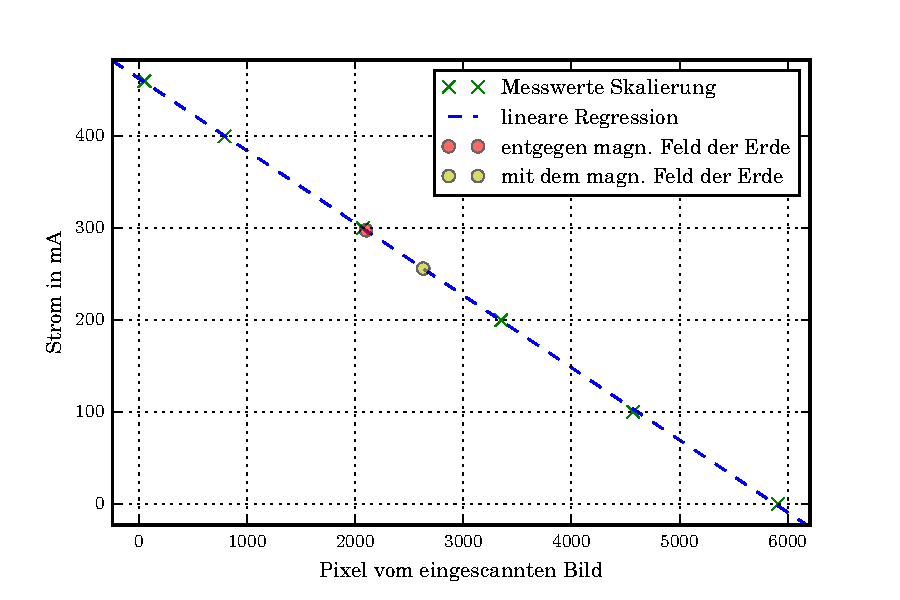
\includegraphics[width=\textwidth]{picture/10MHz.pdf}
     \caption{10.6 MHz}
     \label{fig:10Reg}
  \end{subfigure}
  \begin{subfigure}[b]{0.49\textwidth}
     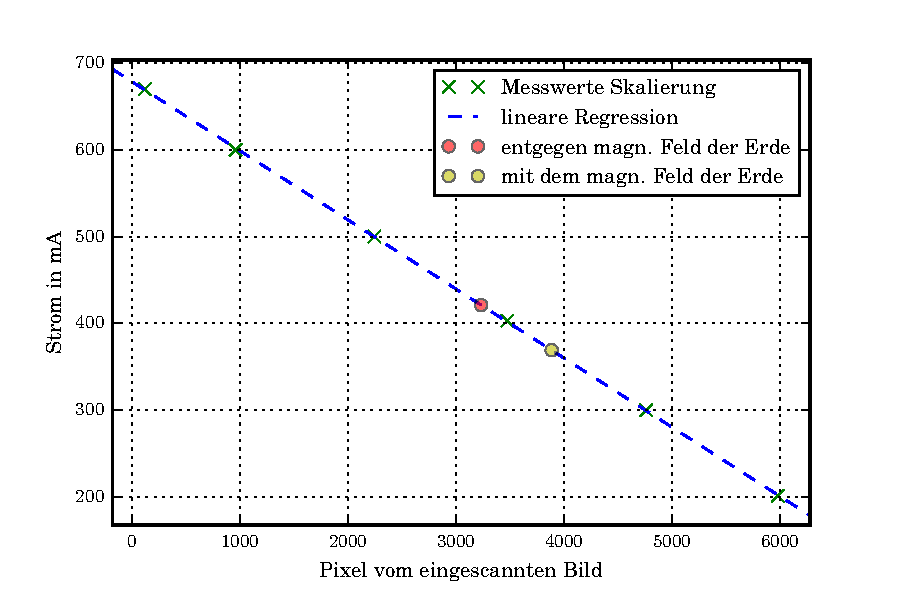
\includegraphics[width=\textwidth]{picture/15MHz.pdf}
     \caption{15.9 MHz}
     \label{fig:15Reg}
  \end{subfigure}
  \begin{subfigure}[b]{0.49\textwidth}
     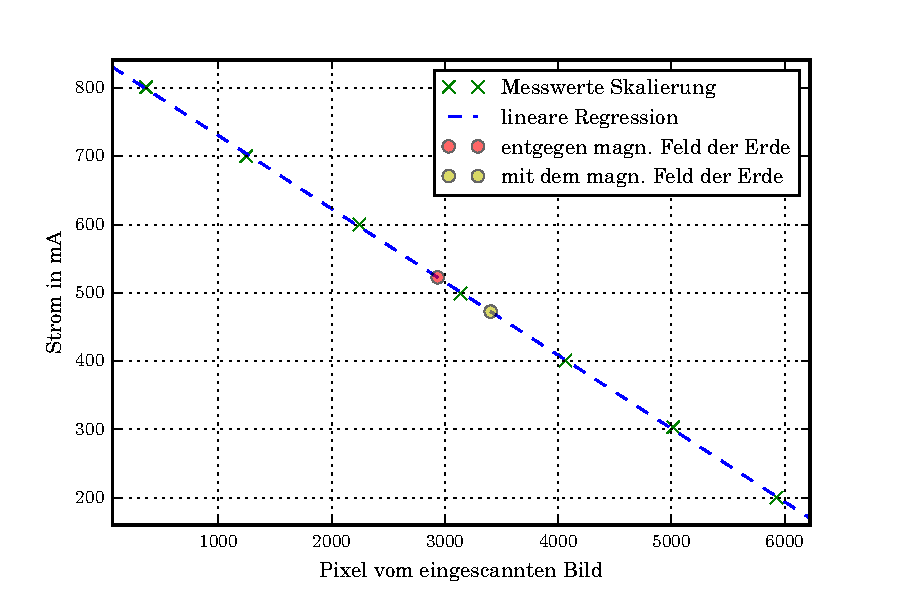
\includegraphics[width=\textwidth]{picture/20MHz.pdf}
     \caption{20.5 MHz}
     \label{fig:20Reg}
  \end{subfigure}
  \begin{subfigure}[b]{0.49\textwidth}
     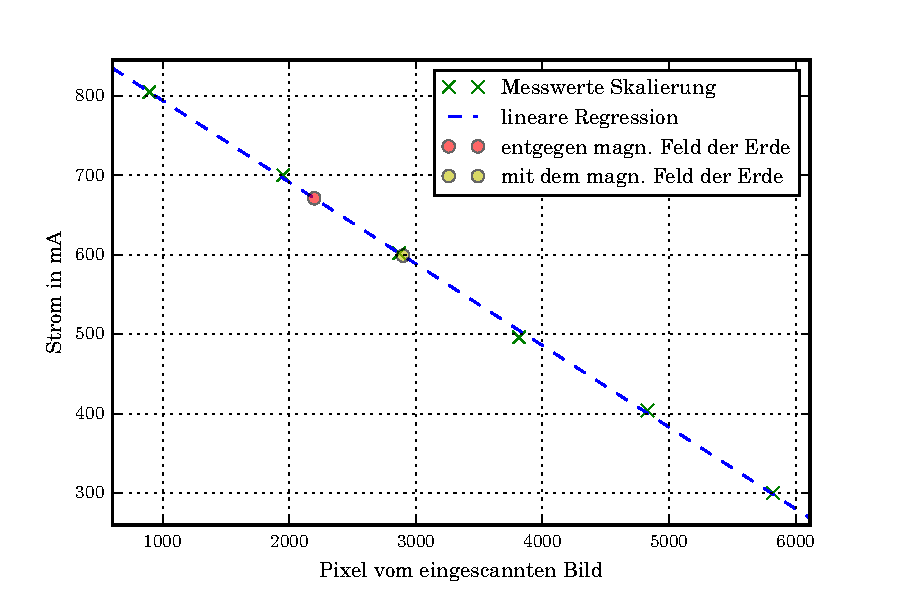
\includegraphics[width=\textwidth]{picture/25MHz.pdf}
     \caption{25.0 MHz}
     \label{fig:20Reg}
  \end{subfigure}
  \begin{subfigure}[b]{0.49\textwidth}
     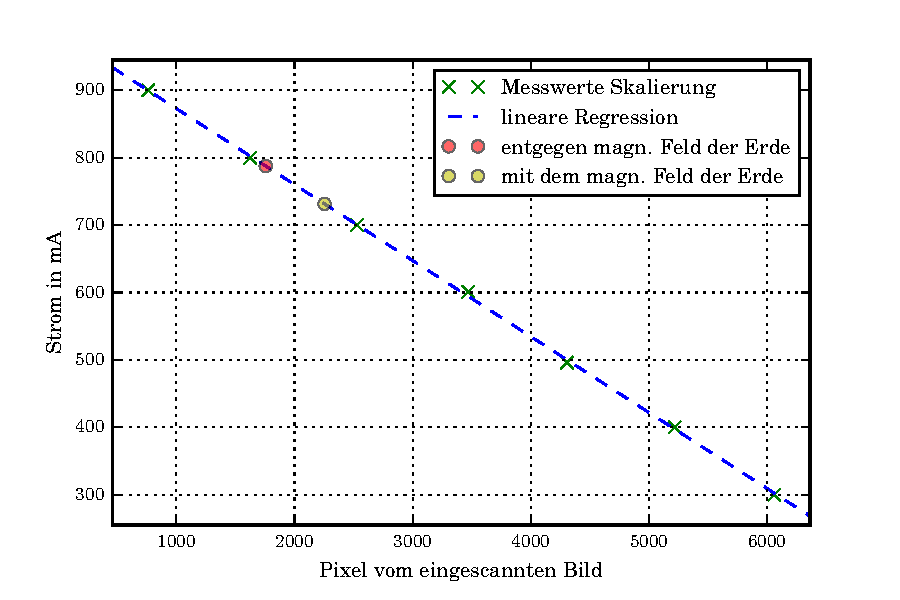
\includegraphics[width=\textwidth]{picture/30MHz.pdf}
     \caption{29.4 MHz}
     \label{fig:30Reg}
  \end{subfigure}
  \caption{Lineare Regression zwischen der Pixel und des Spuelnstroms für unterschiedliche Frequenzen}
  \label{fig:Reg}
\end{figure} 
Anhand der Steigunungen $m$ und der y-Achsenabschnitte $b$ der linearen Regression
\begin{equation}
  f(x) = m \cdot x + b
  \label{eqn:Reg}
\end{equation}
ergeben sich die in Tabelle \ref{tab:stei} aufgeführten Koeffizienten. 
\begin{table}
  \centering
  \caption{Koeffizeienten der linearen Regression}
  \begin{tabular}{c|c c}
    \toprule
    	$\nu_\text{e}$ & Steigung m & Bios b \\
    \midrule
       	10.6 MHz & \num{7.87 +- 0.04}  & \num{463 +- 1.4} \\
	15.9 MHz & \num{7.97 +- 0.03}  & \num{678.6 +- 1.1} \\ 
	20.5 MHz & \num{10.73 +- 0.07} & \num{837 +- 2} \\
	25.0 MHz & \num{10.2 +- 0.1}   & \num{897 +- 5} \\
	29.4 MHz & \num{11.27 +- 0.08} & \num{986 +- 3.3}\\
    \bottomrule
  \end{tabular}
  \label{tab:stei}
\end{table}

\subsection{Bestimmung der Feldstärken}
Aus der zuvor berechneten Regression lassen sich die Spulenströme für den Resonanzfall ermitteln, indem die Extrema der Graphen, welche in Abbildung \ref{fig:Skizze} zu sehen sind, bestimmt werden. Anschließend werden die magnetischen Feldstärken anhand von Formel \ref{eqn:BHelm} berechnet. Die magnetischen Feldstärken, entsprechend gegen und in Richtung des Erdmagentfeldes gerichteten Aufbau, sind in Tabelle \ref{tab:magn} in Abhängigkeit von $\nu_\text{e}$ aufgetragen.  
\begin{table}
  \centering
  \caption{Magnetische Felder in Abhängigkeit der Oszillatorfrequenz}
  \begin{tabular}{c|c c c}
    \toprule
    \multirow{2}{*}{$\nu_\text{e}$} & B-Feld in Richtung & B-Feld entgen der Richtung & gemitteltes \\
    	& des Erdmagnetfeld / $\mu T$ & des Erdmagnetfeld / $\mu T$ & B-Feld / $\mu T$ \\
    \midrule
       	10.6 MHz & \num{417 +- 2} & \num{359 +- 3} & \num{388 +- 2} \\
	15.9 MHz & \num{590 +- 2} & \num{518 +- 2} & \num{554 +- 2} \\ 
	20.5 MHz & \num{733 +- 4} & \num{663 +- 5} & \num{698 +- 4} \\
	25.0 MHz & \num{941 +- 8} & \num{840 +- 8} & \num{891 +- 8} \\
	29.4 MHz & \num{1105 +- 5} & \num{1026 +- 5} & \num{1066 +- 5} \\
    \bottomrule
  \end{tabular}
  \label{tab:magn}
\end{table}
Der Mittelwert aus den beiden Fällen entspricht dementsprechend, den Erdmagnetfeld freien Fall und ist ebenfalls in Tabelle \ref{tab:magn} aufgetragen.
\subsection{Landefaktoren und Erdmagnetfeld}
Ebenso lässt sich aus der halben Differenz der beiden magnetischen Feldstärken das magn. Feld der Erde in Dortmund berechnen. Für die verschiedenen $\nu_\text{e}$ sind diese aufgeführt.
\begin{table}
  \centering
  \caption{Landefaktoren und Stärke des Erdmagnetfeldes}
  \begin{tabular}{c|c}
    \toprule
    	$\nu_\text{e}$ & Erdmagnetfeld / $\mu$ T \\
    \midrule
       	10.6 MHz & \num{29.2 +- 0.2} \\
	15.9 MHz & \num{36.5 +- 0.1} \\ 
	20.5 MHz & \num{35.1 +- 0.2} \\
	25.0 MHz & \num{50.6 +- 0.6} \\
	29.4 MHz & \num{39.4 +- 0.3} \\
    \midrule
	Mittel & \num{38.4 +- 1.5} \\
    \bottomrule
  \end{tabular}
  \label{tab:lande}
\end{table}
Der Landefaktor wird berechnet indem eine weitere Regression durch die Tupel aus gemittelten B-Feld und der Frequenz $\nu_\text{e}$ gelegt wird.
\begin{figure}[htpb]
  \centering
  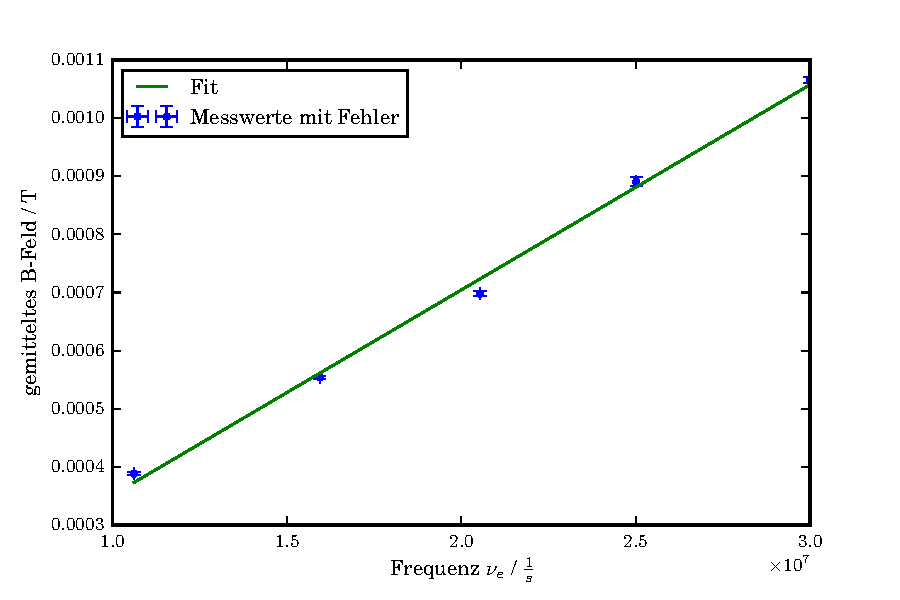
\includegraphics[width=\textwidth]{picture/lande.pdf}
  \caption{Quotient aus dem gemittelten Magnetfeld und der Frequenz $\nu_\text{e}$}
  \label{fig:lande}
\end{figure}
Aus der Steigung der Graden 
\begin{equation}
  m = ??
  \label{<++>}
\end{equation}
wird mittels Formel \ref{eqn:lande} der Land\'{e}-Faktor berechnet. Der Land\'{e}-Faktor beträgt 
\begin{equation}
  g = \num{2.01 +- ??} \ . 
  \label{eqn:landefak}
\end{equation}

